\chapter{Pendahuluan}

Bab Pendahuluan secara umum menceritakan landasan kerja dan arah kerja penulis tugas akhir, yang berfungsi untuk mengantar pembaca dalam memahami dan menganalisis laporan tugas akhir secara keseluruhan. Bab ini terdiri dari latar belakang, rumusan masalah, tujuan, batasan masalah, metodologi, dan sistematika pembahasan tugas akhir.

\section{Latar Belakang}
\label{sec:latarbelakang}

Teknologi dan internet adalah kebutuhan yang penting dalam kehidupan manusia di abad ke-21 ini. Salah satu bentuk teknologi modern paling berguna yang mudah diakses manusia adalah \emph{smartphone}, di mana akses internet sudah termasuk ke dalamnya. Berdasarkan penelitian yang dikumpulkan oleh \textcite{turner2022howmanysmartphones} pada bankmycell.com, pada tahun 2021 terdapat 6.37 miliar pengguna \emph{smartphone} di dunia atau sekitar 80.68\% dari populasi dunia, di antaranya 160.23 juta adalah penduduk Indonesia.

Banyak pekerjaan manusia yang dapat dilakukan dengan menggunakan berbagai jenis aplikasi yang dapat ditemukan dalam sebuah \emph{smartphone}. Menurut penelitian yang dilakukan oleh BusinessofApps, jumlah aplikasi pada iOS App Store ketika pertama kali diluncurkan pada tahun 2008 adalah 500, pada bulan November tahun 2021 angka tersebut melonjak menjadi 1.85 juta aplikasi. Pengguna Android memiliki lebih banyak pilihan dengan total 2.56 juta aplikasi di Google Play Store. Dengan banyaknya aplikasi tersebut, pada tahun 2020 pengguna \emph{smartphone} telah mengunduh aplikasi sebanyak 142.9 miliar kali, di antaranya 56.1 miliar unduhan adalah untuk aplikasi permainan \emph{mobile}.

Teknologi informasi yang semakin berkembang dapat meningkatkan kesejahteraaan digital, atau \textit{digital wellbeing}, dari pengguna teknologi tersebut, beberapa caranya adalah meningkatkan koneksi sosial, mendukung kesehatan mental, dan mendukung kebiasaan sehat dengan fleksibilitas dalam praktik kerja. Namun teknologi informasi juga dapat menimbulkan akibat buruk yang memunculkan pola penggunaan teknologi yang tidak sehat. Beberapa contoh dampak buruk yang dimunculkan adalah mudahnya seseorang untuk kehilangan fokus, perasaan \emph{fear of missing out} (FoMO), serta kecanduan digital. Sifat-sifat buruk tersebut dapat lebih sering muncul ketika waktu yang dihabiskan pada dunia maya tidak diimbangi dengan waktu di dunia nyata \parencite{ALMOURAD2021101778}.

Pengaruh buruk seperti yang telah disebutkan di atas serta perilaku adiksi pada \textit{smartphone} telah memunculkan perhatian bagi peneliti di bidang \textit{Human Computer Interaction} (HCI) untuk melakukan studi terhadap kesengajaan untuk tidak menggunakan teknologi. Studi tersebut memunculkan sebuah konsep "\textit{Digital Wellbeing}" yang berfokus dalam peningkatan kesejahteraan pengguna dalam pemakaian media digital \parencite{unesco2015dwconference}. Pada saat ini, terdapat banyak perangkat lunak pada \textit{smartphone} yang menerapkan konsep tersebut untuk mengubah perilaku penggunanya, salah satunya dibuat oleh Google \parencite{CHI2019SOCIALIZE}. Untuk membantu penggunanya, Google merilis aplikasi dengan nama yang sama, Digital Wellbeing, agar pengguna dapat memanfaatkan teknologi untuk meningkatkan kualitas kehidupannya melainkan menjadi distraksi. Pada websitenya tentang Digital Wellbeing, \textcite{google2019digitalwellbeing} mengatakan: "We’re committed to giving everyone the tools they need to develop their own sense of digital wellbeing. So that life, not the technology in it, stays front and center." 


\section{Rumusan Masalah}

Penggunaan tinggi \textit{smartphone} dapat mempengaruhi kesejahteraan digital dari penggunanya dalam cara yang negatif. Salah satu bentuk dari hubungan yang tidak baik antara \textit{smartphone} dan penggunanya adalah tingginya tingkat ketergantungan terhadap \textit{smartphone} hingga dapat mencapai tingkat adiksi. Penurunan kualitas hubungan tersebut dapat disebabkan oleh gangguan distraksi dari aplikasi pada \textit{smartphone} atau keinginan pengguna sendiri untuk menggunakannya. Dalam upaya memperbaiki hubungan tersebut, Google merilis aplikasi Digital Wellbeing yang bertugas untuk membantu pengguna \textit{smartphone} berbasis Android untuk mengatur kesehatan penggunaannya. Namun, dengan banyaknya aplikasi dengan tujuan serupa di \textit{marketplace} Google Play Store, dapat dilihat bahwa terdapat beberapa batasan pada aplikasi Digital Wellbeing. Maka dari itu, dapat disimpulkan rumusan masalah yang akan didalami dalam tugas akhir ini adalah sebagai berikut

\begin{enumerate}
  \item Apa \textit{usability goals} dan \textit{user experience goals} yang tepat untuk sebuah aplikasi pencegah distraksi?
  \item Apa fitur-fitur dan desain interaksi yang diperlukan untuk menyelesaikan masalah dari aplikasi pencegah distraksi Google Digital Wellbeing yang dirancang menggunakan pendekatan \textit{user-centered design}?
  % \item Bagaimana rancangan desain interaksi yang tepat untuk menyelesaikan masalah yang terdapat pada aplikasi pencegah distraksi Digital Wellbeing?
  % \item Bagaimana prototipe aplikasi pencegah distraksi Digital Wellbeing dengan desain interaksi menggunakan pendekatan \emph{user-centered design}?
\end{enumerate}

\section{Tujuan}

Berdasarkan latar belakang dan rumusan masalah di atas, tujuan dari tugas akhir ini adalah untuk membuat sebuah prototipe aplikasi pencegah distraksi. Prototipe aplikasi tersebut memiliki desain interaksi yang dapat menyelesaikan masalah-masalah desain interaksi yang ditemukan pada aplikasi Digital Wellbeing.


\section{Batasan Masalah}

Batasan masalah untuk implementasi solusi tugas akhir ini adalah sebagai berikut
\begin{enumerate}
  % \item Hasil akhir dari studi adalah solusi dalam bentuk prototipe aplikasi untuk \textit{smartphone} berbasis Android dengan versi OS lebih besar sama dengan versi Android 9.0.
  \item Responden penelitian adalah masyarakat Indonesia, dengan rentang umur 18 hingga 30 tahun.
  \item Hasil akhir dari studi adalah solusi dalam bentuk prototipe \textit{high-fidelity} desain interaksi aplikasi yang didesain untuk \textit{smartphone} berbasis Android.
  % \item Pengujian akan dilakukan dengan membandingkan penggunaan \textit{smartphone} yang disertai bantuan aplikasi Digital Wellbeing dengan prototipe aplikasi solusi.
\end{enumerate}

\section{Metodologi}
\label{sec:metodologi}

Metodologi dalam perancangan solusi tugas akhir menggunakan pendekatan \textit{user-centered design} (UCD) yang mengikuti standar alur kerja dari ISO (\textit{International Organization for Standardization}) 9241-210:2010. Berikut adalah penjelasan dari setiap tahap UCD sesuai dengan yang tertera pada Diagram UCD dalam Gambar \ref{fig:diagram_iso1}


\begin{figure}[h]
  \centering
  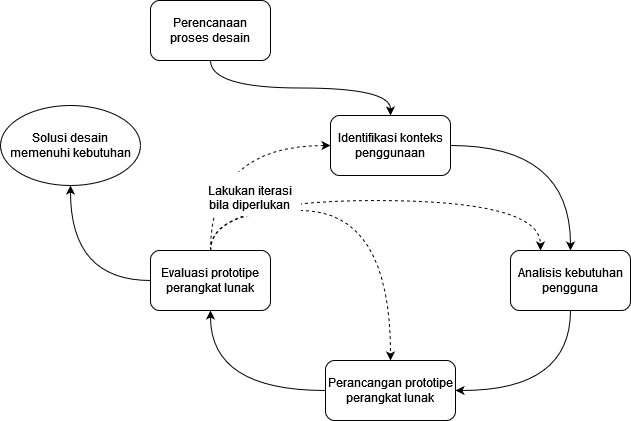
\includegraphics[width=0.9\textwidth]{chapter-1-method.png}
  \caption{Diagram alur pengerjaan \textit{User-Centered Design} (ISO 9241-210, 2010)}
  \label{fig:diagram_iso1}
\end{figure}

\begin{enumerate}
  \item Perencanaan proses desain
  \subitem Proses UCD diawali dengan tahap persiapan, yaitu proses penentuan terhadap lingkup aplikasi yang dibuat serta perencanaan untuk pengambilan data. Lingkup dari aplikasi termasuk jenis antarmuka dan \textit{platform} yang dipilih untuk implementasi, lingkup fungsionalitas aplikasi, serta target pengguna aplikasi. Sedangkan perencanaan pengambilan data dilakukan dengan cara analisis ulasan aplikasi dan wawancara pengguna.

  \item Identifikasi konteks penggunaan
  \subitem Pada tahap ini dilakukan pengumpulan data pengguna melalui analisis ulasan pengguna dan wawancara sesuai dengan kebutuhan. Data yang didapatkan akan dianalisis untuk mengungkapkan perilaku dan permasalahan pengguna tentang aplikasi. Fungsionalitas dari aplikasi juga penting untuk mengerti konteks penggunaannya. Berdasarkan data riset tersebut akan dibentuk persona pengguna, yang kemudian akan dianalisis untuk mendapatkan kebutuhan, tujuan dan kegiatan pengguna, serta skenario pengguna.
   
  \item Penentuan kebutuhan perangkat lunak
  \subitem Tahap ini terdiri dari analisis prinsip desain, analisis \textit{usability goals} dan \textit{user experience goals}, analisis tipe interaksi, serta analisis fitur. Fitur-fitur hasil analisis dipetakan ke dalam halaman dan \textit{widget} yang diperlukan. Dilakukan juga analisis \textit{user flow} merancang alur penggunaan aplikasi. Hasil-hasil analisis yang terkumpul akan menjadi bahan implementasi pada tahap selanjutnya.
  
  \item Perancangan prototipe perangkat lunak
  \subitem Rancangan kebutuhan pengguna yang sudah dikumpulkan pada tahap sebelumnya akan kemudian diimplementasikan, mulai dari \textit{low-fidelity prototype}, dilanjut dengan \textit{high-fidelity prototype}. Proses ini dilakukan secara iteratif bersamaan dengan tahap evaluasi.
  
  \item Evaluasi prototipe perangkat lunak
  \subitem Tahap evaluasi dilakukan untuk menguji kemampuan solusi desain yang telah dirancang dalam memenuhi kebutuhan pengguna dan \textit{user experience goals} serta \textit{usability goals} yang ditargetkan. Hasil evaluasi menentukan apakah desain yang diuji perlu diperbaiki dalam proses iterasi.

  
\end{enumerate}


\section{Sistematika Pembahasan}

\begin{enumerate}
  \item Bab I Pendahuluan
  \subitem Bab I adalah pendahuluan yang berisi latar belakang dari pengerjaan tugas akhir, rumusan masalah yang ingin diselesaikan, tujuan yang ingin dicapai, batasan masalah yang ditentukan, metode yang digunakan selama proses pengerjaan, serta sistematika pembahasan tugas akhir.
   
  \item Bab II Studi Literatur
  \subitem Bab II membahas tentang studi literatur sebagai landasan teori untuk bab III dan bab IV. Pada bab ini, dituliskan hasil studi literatur terhadap adiksi smartphone, Digital Wellbeing, desain interaksi, \textit{usability testing}, serta penelitian terkait tugas akhir.
 
  \item Bab III Identifikasi Masalah dan Rancangan Solusi
  \subitem Bab III membahas proses identifikasi masalah dan perancangan solusi yang akan dibentuk. Bab ini memuat tiga tahap pertama dari metodologi \textit{user-centered design}, yaitu perencanaan proses desain, identifikasi konteks masalah, dan penentuan kebutuhan perangkay lunak.
 
  \item Bab IV Implementasi dan Pengujian Prototipe
  \subitem Bab IV memuat tahap lanjutan dari \textit{user-centered design}, yaitu perancangan prototipe perangkat lunak serta evaluasi prototipe perangkat lunak. Pada bab ini, kedua tahap tersebut mengalami iterasi, diawali dengan implementasi dan pengujian prototipe \textit{low-fidelity}, implementasi dan pengujian prototipe \textit{high-fidelity} iterasi pertama, serta implementasi dan pengujian prototipe \textit{high-fidelity} iterasi kedua yang ditetapkan sebagai solusi desain yang memenuhi tujuan tugas akhir. Adapun tahap analisis kelayakan implementasi yang dilakukan setelah proses UCD selesai untuk memastikan bahwa desain yang dirancang dapat diimplementasikan.
 
  \item Bab V Kesimpulan dan Saran
  \subitem Bab V memaparkan kesimpulan dari proses perancangan prototipe desain solusi tugas akhir. Bab ini juga memuat saran mengenai hal yang dapat dilakukan ke depannya untuk memperbaiki solusi yang dibuat pada tugas akhir ini.
\end{enumerate}